\documentclass[12pt, letterpaper]{article}

% Packages for formatting and aesthetics
\usepackage{tikz}
\usepackage{amsmath}
\usepackage{geometry}
\usepackage{parskip}          % For better spacing between paragraphs
\usepackage{microtype}        % For better typography
\usepackage{lmodern}          % For a cleaner, more modern font
\usepackage{titlesec}         % To customize section titles
\usepackage{setspace}         % For line spacing
\usepackage{fancyhdr}
\pagestyle{fancy}
\fancyfoot[L]{SPT-16}

% Custom geometry settings
\geometry{
    top=1in,
    bottom=1in,
    left=1.25in,
    right=1.25in
}

% Line spacing
\onehalfspacing

% Title format customization
\titleformat{\section}{\large\bfseries}{\thesection}{1em}{}
\titlespacing*{\section}{0pt}{2em}{1em}

\title{\vspace{-2cm}Évariste} % Reduce the space before the title
\author{Himanshu, Taraash, Rachit, Farhan}
\date{November 6, 2024}

\begin{document}
\maketitle

\section*{Speed Proving Tournament}
SPT is a knockout round problem solving competetion where one team tackles a given problem on the blackboard while others do it on piece of paper, the first team to solve one with get half a point (one if done on the board).


\section{GEOMETRY}
\begin{enumerate}
        \item The sides AD and BC of a convex polygon are extended to meet at E. Let H and G be the midpoints of BD and AC respectively. Find the ratio of the area of the triangle EGH to that of the quadrilateral ABCD.
    
    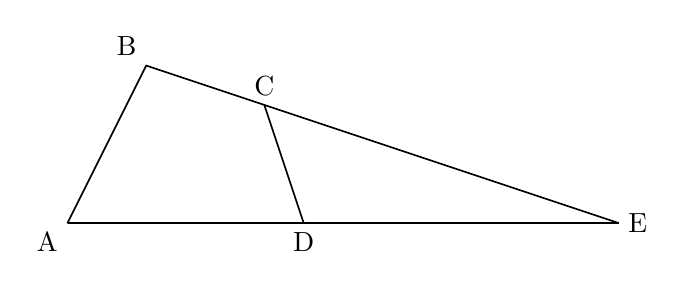
\begin{tikzpicture}
        \draw[line width=0.6pt] (0, 0) -- (1, 2) -- (2.5, 1.5) -- (3, 0) -- (0, 0);
        \draw[line width=0.6pt] (2.5, 1.5) -- (7, 0);
        \draw[line width=0.6pt] (3, 0) -- (7, 0);
        \node[below left] at (0, 0) {A};
        \node[above left] at (1, 2) {B};
        \node[above] at (2.5, 1.5) {C};
        \node[below] at (3, 0) {D};
        \node[right] at (7, 0) {E};
    \end{tikzpicture}
\end{enumerate}

\section{NUMBER THEORY}
\begin{enumerate}
    \item 3 more than the \emph{concatenation of two \emph{(not necessarily distinct) primes }q and r} is the square of a prime \emph{p}. Find all possible values of \emph{p}. \emph{(for example, if q = 7 and r = 17, the concatenation of q and r is 717).}
\end{enumerate}


\section{ALGEBRA}
    
\begin{enumerate}
    \item $P(x)$ is a 4th degree polynomial with real coefficients such that $P(x) \geq x$.
    $P(1) = 1$, $P(2) = 4$, $P(3) = 3$.
    Find the value of $P(4)$.
    
    \item The coefficients of the polynomial \emph{P(x)} are non-negative integers, each less than 100. Given that
    P(10) = 331633 and \(P(-10) = 273373\), compute P(1).
    
\end{enumerate}

\section{PIGEONHOLE PRINCIPLE}
\begin{enumerate}
    \item A chess master who has 11 weeks to prepare for a tournament decides to play at least one game every day, but, in order not to tire himself, he decides not to play more than 12 games during any calendar week. Show that there exists a succession of consecutive days during which the chess master will have played exactly 21 games.

\end{enumerate}


\vspace{100pt}
% Floral pattern at the end of the document
\begin{center}

\begin{tikzpicture}
  \draw[scale=0.5,domain=0:360,smooth,variable=\t] plot(\t:{sin(10*\t)});
  % \node at (0,0) {\Huge \textbf{End of the Question Paper}};
\end{tikzpicture}
\end{center}





\end{document}


